\section*{Experimental Setup}
This section focuses on the physical Mu3e experiment. Initially to describe the physical signal of the experiment but also the means by which this signal is measured.

\begin{figure}
    \centering
    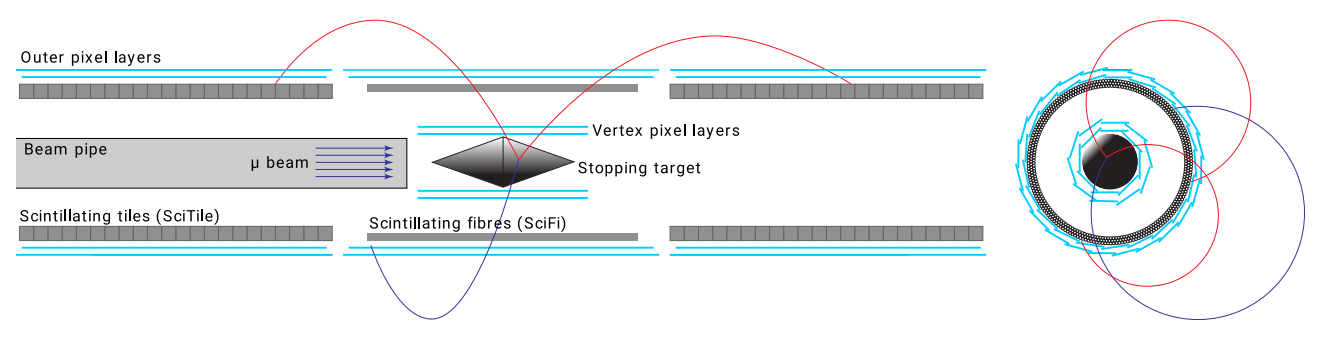
\includegraphics[width=\textwidth]{fig/setup/det.PNG}
    \caption{Figure the layout of the detectors of the Mu3e experiment in the $r-z$ plane, with an example of a $\mu^{+}\xrightarrow{}e^{+}e^{+}e^{-}$ decay \cite{rudzki2021mu3e}.}
    \label{fig:det}
\end{figure}

\subsection*{Beam and Stopping Target}
Phase 1 of the experiment will use the Compact Muon Beam Line (CMBL) based at PSI as this is the only muon beam capable of generating the high rate of muons required to reach the desired sensitivity of the experiment. PSI has a $1.4$MW proton beam which delivers protons of $590$MeV at a current of $2.4$mA \cite{kiselev2021meson} to target E, in the case of Mu3e. Through interactions with the protons in the nuclei of the target material, pions are produced in abundance\cite{berg2016target}. The type of pion produced with the largest abundance is the positive pion and therefore these are selected, and the rest of the decay products are filtered. Of these positive pions, those that have been stopped on the target are selected as they decay to surface muons with enough energy to escape the surface of the target. The reason for selecting these surface muons as opposed to the muons that are generated around the target as well is that they are almost always the same charge \cite{berg2016target}, have a small momentum range and are $\simeq 100\%$ polarized\cite{kiselev2021meson}. Specifically the low momentum of these surface muons allows for accurate control of their momentum and therefore ideal for stopping on thin targets, as is the case in Mu3e. The beam generates close to $10^{8}\mu^{+}/s$ \cite{Calibbi}. This beam is shared between Mu3e and the MEG II experiment. 

\paragraph{}
 The muons from the CMBL are directed to the stopping target situated at the centre of the central station of the Mu3e experiment as shown in figure \ref{fig:det}. The target is a double cone shape as shown in figure \ref{fig:stop}. The purpose of the target is to stop muons in the center of the tracker. By doing this, the initial vertex can be reconstructed from one stationary point and the sum of the momenta of the reconstructed tracks should be equal to zero. The sum of the magnitudes of the momentum of the tracks should also equal the invariant mass of the muon. The final design of the stopping target is given in figure \ref{fig:stop}. Two factors were the focus of the design of the stopping target: maximising stopping power and spreading the decay vertices out as much as possible. In order to maximise stopping power, the amount material in the z-direction needs to be increased as much as possible. This however had to be balanced with the need to minimise material in the way of the tracks to reduce multiple scattering. The other factor was to spread the vertices out as much as possible, this allows for a low occupancy in local areas of the pixel detector and to reduce combinatorial background by decreasing the number of coincidental vertices \cite{Arndt}. The combination of these factors led to the hollow, double cone shape as seen. This design best satisfies these requirements as the angle of the cone allows for the vertices to be spread out along the surface which distributes the decay tracks evenly across the detector. The use of $70-80\mu m$ Mylar allows for minimal photon conversion and multiple scattering which is the largest background source for Mu3e.

\begin{figure}
    \centering
    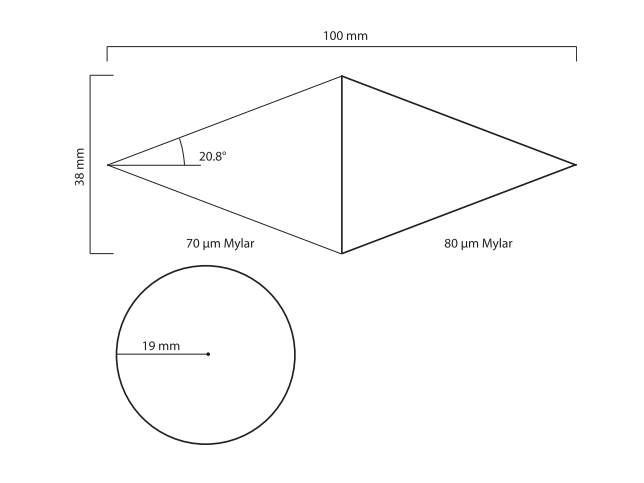
\includegraphics[width=\textwidth]{fig/setup/stop.PNG}
    \caption{Figure showing the dimensions of the stopping target. The upper image is from the $r-z$ plane, the lower from the $x-y$ plane. For the upper image the beam would be incident on the left side of the target \cite{Calibbi}.}
    \label{fig:stop}
\end{figure}

\subsection*{Magnet}
The purpose of the magnet is for particle identification and precise momentum measurements. By having the detector sat inside a magnetic field, the charged decay products are forced into helices that are dependant on their respective charge and momentum. Positrons are propagated in the negative z-direction and electrons in the positive. This field also forces the decay products into helices which allows for longer tracks to be generated. This in turn allows for precise measurements of the momentum as more spatial and temporal information can be collected. The field drives the tracks through the central station and then back into one of the two recurl stations that sit up and downstream of the central detector. In order to achieve the precision required by Mu3e, the chosen magnet is a superconducting $1T$ solenoidal magnet. This must also have an inhomegeniety of $\leq 10^{-3}$ and a stability over 100 days of $\leq 10^{-4}$ \cite{Arndt}.

\subsection*{Scintillating Fibres and Tiles}
Scintillating fibres and tiles are used to provide timing information of the tracks. The suppression of combinatorial background is essential for Mu3e, this is achieved with excellent vertex resolution which in turn is dependant on the timing resolution. As Mu3e uses tracks that recurl back into the detector to gain precise measurements of the momentum, the timing detectors are therefore used to reduce ambiguity in the direction of the tracks as there will be a time difference between tracks exiting and entering the detector. The charge of the decay products can also be identified by the timing detectors. This can be achieved with time of flight measurements and the direction these measurements are taken. Hits in the fibres can be causally related to hits in the tiles and vice versa to identify a common track. Using the spacial information from the timing detectors in combination with the knowledge of the direction of the magnetic field will give charge identification. The timing resolution of the pixel sensors is $\leq 20 ns$ which when combined with the readout time creates event frames that are $64 ns$ (CHECK) long. In order to identify charge a timing resolution of $\leq 500 ps$ is required. In order to temporally separate muon decays in the same frame a resolution of $\leq 100 ps$ is required \cite{Arndt}.

\subsubsection*{Scintillating Fibres}
The scintillating fibres in the central detector are arranged into a series of ribbons that are placed in between the second and third silicon tracking layers. They provide a timing resolution of $250 ps$ with a signal efficiency of $96 \%$ and spatial resolution of $\sim 100 \mu m$ \cite{bravar2022development}. To minimise the effects of multiple scattering and energy loss, the fibres are arranged into ribbons comprised of three layers of $250 \mu m$ thick fibres. This lowers the percentage of the radiation length to $< 0.2\% X\backslash X_{0}$. The primary purpose of the scintillating fibres is separate individual events in frames recorded by the silicon tracker. The secondary is to use time of flight information, as tracks either recurl into the central station or into the recurl stations, to identify the charge of the particle being measured.

\subsubsection*{Scintillating Tiles}
Located in the recurl stations are the tile detectors. 
The tile detectors are arranged in a hollow cylinder, just like the scintillating ribbons. 
As tiles are placed in the recurl stations, they provide timing on the end of tracks and therefore scattering effects and energy loss is not a concern. 
This means a much more efficient material can be used. The material is a $6.3 \times 6.2 \times 5.0 mm^{3}$ plastic scintillator. 
Due to the higher photon yield, the detector efficiency is much higher than the fibres. After calibration, the efficiency was found to be above $99\%$. 
The requirement of the tiles is to have a timing resolution of $\leq 100ps$ \cite{Arndt}, but after testing it was shown the single channel timing resolution was $\approx 47 ps$ \cite{klingenmeyer2020measurements}.

\subsection*{Silicon Trackers}
The silicon tracking layers are used to provide spatial information on the tracks left by the decay products. 
Like the timing detectors, these pixel layers are hollow cylinders arranged concentrically around the beam line. 
These layers in turn are made up of a series of pixel sensors fixed to ladders that lie parallel to one another. 
The sensors themselves are high voltage monolithic active pixel sensors (HV-MAPS) that utilise CMOS technology. 
By using CMOS technology amplification of the signal is done for each pixel individually as seen in figure \ref{fig:pix}. 
Unlike MAPS, HV-MAPS collect charge (deposited by a particle passing through the depletion region) using drift rather than diffusion which allows for much higher time resolution, a critical factor for the Mu3e experiment \cite{schoning2020mupix}. 
The voltage is determined by the resistivity, which in turn is largely determined by the depth of the depletion region. 
This can be thinned to $15-50 \mu m$ which means the total depth of the sensor can be extremely small. 
The thinner the sensor, the amount of material in the decay products path is reduced and therefore the effect of multiple scattering is reduced. 
For phase one of Mu3e, the sensors will be thinned to $50 \mu m$. A final key feature of the sensors for Mu3e is their use of two comparators in parallel in the periphery electronics of the pixel as seen in figure \ref{fig:pix}. 
By doing this two separate signal thresholds can be set, a lower threshold for time information/sampling and a higher threshold for hit validation \cite{augustin2021mupix10}. 
By having these two pieces of information, it allows for low noise (by validating the signal) and low jitter (by using the time information) \cite{schoning2020mupix}. 
The final prototypes of the MuPix sensors showed a hit efficiency of $>99\%$ efficiency \cite{rudzki2021mu3e}.

\begin{figure}
    \centering
    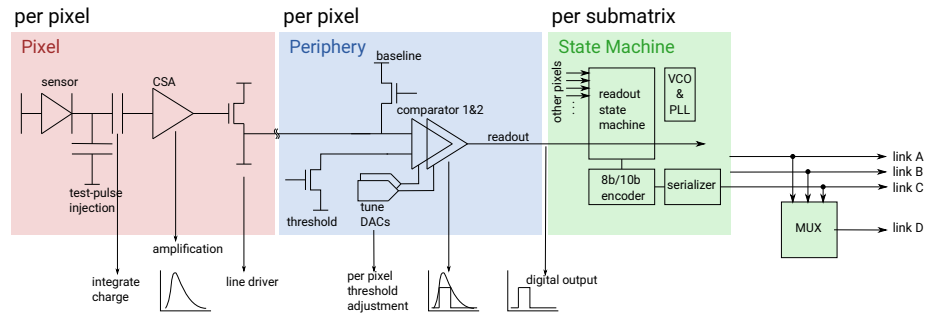
\includegraphics[width=\textwidth]{fig/setup/pix.PNG}
    \caption{Figure showing the pixel architecture for MuPix10 \cite{augustin2021mupix10}.}
    \label{fig:pix}
\end{figure}

\paragraph{}
The arrangement of the pixel tracking layers are shown in figure \ref{fig:det}. 
The two innermost layers are the vertex locator, following from there are the outer layers: two layers in the central detector, and two layers in each recurl station. 
The purpose of the layers is to collect hits from the decay products and provide spacial and temporal information on these hits.

\section*{Tracking in the Mu3e Experiment}
The Mu3e experiment sits in a homogenous solenoidal magnetic field centered around the z-axis. In this setup, a right-handed coordinate system is used with the z-axis sat parallel to the direction of the magnetic field. 
This setup forces the decay products into a characteristic helix, from which the momenta and thus the energy of these particles can be derived.
As stated, calculation of the momenta of the tracks, in conjunction with the geometrical properties of the decay vertex, are used to identify potential signal events.
The physical background events are internal conversion. In order to discriminate these background events from signal an excellent momentum resolution is required (1 Mev \cite{MartinPerez2023}).
\subsection*{Geometrical Foundation of Tracking}
The charged products of the signal decay are forced into helices by the magnetic field centered on the z-axis of the experiment.
By parameritising the geometrical properties of a given helix, spatial information of hits in the detector can be used to draw the shape of the tracks of these products and thus energy and momenta can be calculated.
The first task is to factorise out the circular fit of the tracks in the x-y plane and the linar fit in the z axis.
From the basic fit of a helix, the uncertainty due to multiple scattering is incorporated.
The parameterisation of the helices follows the method given by \cite{KARIMAKI1991187} and visualised in figure \ref{fig:bend}. 
As seen in figure \ref{fig:bend} three points are taken in successive silicon tracking layers, through which an arc can be drawn.
From this arc, an uncertainty must be introduced due to multiple scattering as the particle passes through the tracking layers.
By assuming momentum is conserved, the radius of curvature is constant and all that must be calculated is the spatial difference between the two centres of the arc.
By calculating this difference, a corrective angle due to multiple scattering can be derived, as denoted in figure \ref{fig:bend} by $\Phi_{MS}$.
By applying a straight line fit in the $s-z$ plane to construct a total helix, a corresponding corrective angle can be applied for the perpendicular plane, given by $\Theta_{MS}$.
In the Mu3e experiment, only the uncertainty due to multiple scattering is taken into account. This therefore leads to the challenge of finding a three-dimensional curvature that minimises equation \ref{eq:chi2}
\begin{equation}
    \chi^{2}(R_{3D}) = \frac{\Phi_{MS}(R_{3D})^2}{\sigma_\phi^2} + \frac{\Theta_{MS}(R_{3D})^2}{\sigma_\theta^2}
    \label{eq:chi2}
\end{equation}
The radius of this arc is denoted with $r$ and the opening angle between the first and last hit is given by $\Phi$.
By introducing bending angles and corrective parameters from multiple scattering each pair of hits has an associated radius and and centre.
To construct larger tracks, a series of triplets that share hits in the silicon trackers are combined. The $\chi^2$ function of the longer tracks is the summation of the $\chi^2$ equation \ref{eq:chi2} for each of the constitiuent triplete due to each scatter being independant of each other.
In practice, the procedure is to collect all the relevant hits for a given track, fit each triplet individually and then calculate the summation of these $\chi^2$ values. Throughout the process of finding relevant hits, selection cuts are applied to the track.
These selection cuts are initially focused on the spatial position of the successive hits, from this a cut is applied on the tangential radius. After the fitting has been completed for the track a cut is made on the $\chi^2$ value.
Every track that passes this set of criteria is passed to the vertex fitter.
\begin{figure}
    \centering
    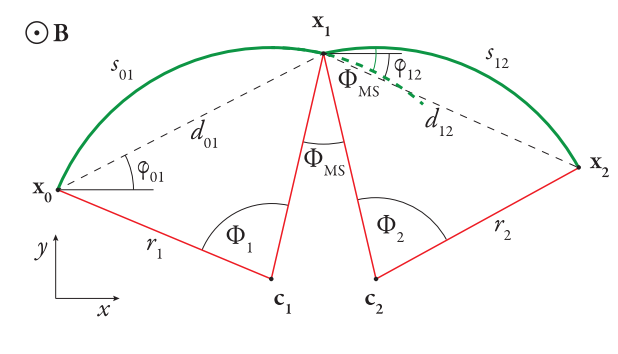
\includegraphics[width=10cm]{fig/tracking/bending.PNG}
    \caption{Figure visualising the tracking parameters associated with the circular fit in the x-y plane. Where $r$ denotes the radius of the arc, $c$ denotes the centre of the arc and $\Phi$ is the opening angle of the arc. \cite{berger2017new}.}
    \label{fig:bend}
\end{figure}